\subsection{Dense-Captioning Events in Videos}

\subsubsection{Overview}

\par Ranjay Krishna \textit{et al}, in their 2017 paper titled \textit{Dense-Captioning Events in Videos} \cite{krishna2017densecaptioning}, proposed the problem of \textit{dense video captioning}. The network was able to output overlapping events and events with varying time scales. The captioning module output also considered past and future context of the representative event. They also introduced new datset with over 20K annotated videos for this problem - ActivityNet Captions.


\subsubsection{Datasets}
\begin{itemize}
\item ActivityNet Captions
\end{itemize}

\subsubsection{Performance}
\par Krishna \textit{et al} compared captioning results with LSTM-YT\cite{venugopalan2015sequence}, S2VT\cite{venugopalan2015translating} and H-RNN\cite{yu2016video} using BLEU@1-4, METEOR and CIDEr. Since these models were only for captioning, the results were compared by providing ground-truth proposal boundaries. The metrics showed better results even when their pipeline generated captions on learnt proposals. The model was tested with different type of contexts input in captioning model, and full-context (\textit{both past and future}) proved to better for longer videos. The results of event localization depicted how multi-stride network performed better for videos with more number of events. The model also reported state-of-the-art results for the task of vdeo and paragraph retrieval


\subsubsection{Methodology}

\par Krishna \textit{et al} architecture consists of two main components:
\begin{enumerate}
	\item Event proposal module
	\item Captioning module with context
\end{enumerate}

\begin{figure}[h]
	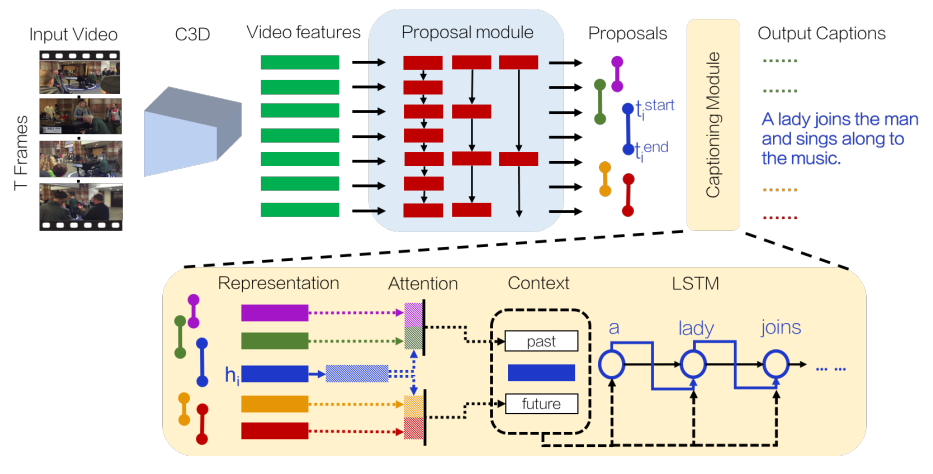
\includegraphics[width=\linewidth]{assets/img/krishna2017densecaptioning-architecture.png}
	\caption{Pipeline introduced by Krishna \textit{et al} (Image courtesy \cite{krishna2017densecaptioning})}
\end{figure}

\paragraph{Flow of pipeline}
\begin{enumerate}
	\item C3D features of sampled video frames.
	\item Sampling done at different strides to capture all kind of events.
	\item Features fed into LSTM type of network inspired by DAPs\cite{Escorcia2016DAPsDA} for generating proposals.
	\item Captioning module used a LSTM network with following inputs:
	\begin{enumerate}
		\item hidden representation of past events $h_i^{past}$
		\item hidden representation of current event $h_i$
		\item hidden representation of future events $h_i^{future}$
	\end{enumerate}
\end{enumerate}


\subsubsection{Conclusion}

\par Krishna \textit{et al} tackled the task of captioning videos with correlation between events. They also showed the results on streaming videos with current event relating to only past events.